\chapter{Evaluation}
\section{Requirement verification}
The top level requirements were already defined at the beginning of the project. In the end of the project it was verified whether the requirements were fully fulfilled, partially fulfilled or not fulfilled (See \autoref{tab:reqverif}). Some of the requirements have to be confirmed (TBC), since the result can only be stated after first launch.
\begin{figure}[H]
	\centering
	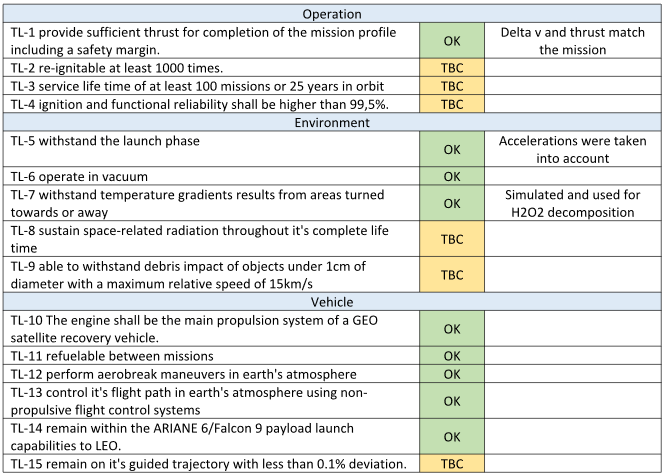
\includegraphics[width=0.85\linewidth]{reqveh}
	\caption{Requirements for the vehicle}\label{tab:reqverif}
\end{figure}

\section{Lessons learnt}
At the end of the project, a lessons learned session was performed to summarize the major problems and issues
during the whole project work. The result can be found in \autoref{fig:lesson}.
\begin{figure}[H]
	\centering
	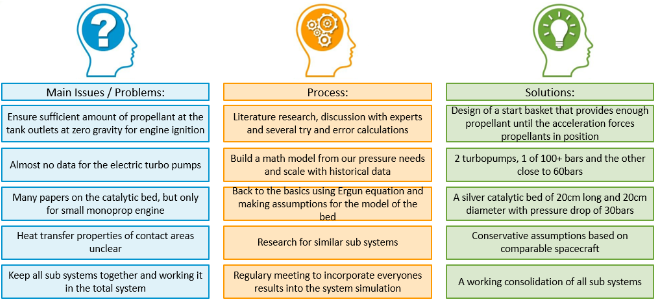
\includegraphics[width=\linewidth]{lessonlearnt}
	\caption{Lessons learnt}\label{fig:lesson}
\end{figure}